% Created 2019-04-16 Tue 22:54
% Intended LaTeX compiler: pdflatex
\documentclass[12pt]{article}
\usepackage[utf8]{inputenc}
\usepackage[T1]{fontenc}
\usepackage{graphicx}
\usepackage{grffile}
\usepackage{longtable}
\usepackage{wrapfig}
\usepackage{rotating}
\usepackage[normalem]{ulem}
\usepackage{amsmath}
\usepackage{textcomp}
\usepackage{amssymb}
\usepackage{capt-of}
\usepackage[hidelinks]{hyperref}
\usepackage{float}
\topmargin 0mm \oddsidemargin 2mm \evensidemargin 2mm \textwidth 160mm \textheight 578.201 pt

\author{Guido España, Alex Perkins}
\date{\today}
\title{Cost-effectiveness of Dengvaxia in Puerto Rico}
\begin{document}

\maketitle

\section{Introduction}
The latest results of the CYD-TDV vaccine show an increased risk of severe dengue upon infection among vaccinees without previous exposure to dengue virus (DENV) \cite{Sridhar2018}. The World Health Organization (WHO) recommends a pre-vaccination screening to ensure that only those with previous exposure to DENV are vaccinated \cite{WHO2018}. However, rapid diagnostic tests with high sensitivity and specificity are not currently available. We have previously discussed the benefits and cost-effectiveness of pre-screening vaccination for economic scenarios of the Philippines and Brazil \cite{Espana2019Biorxiv}. Here, we discuss the implications of this strategy for Puerto Rico in terms of epidemiological benefits and cost-effectiveness. 

\section{Methods}
We updated our assumptions of treatment of dengue for ambulatory cases and hospitalizations, based on estimates from 2002 to 2010 \cite{Halasa2012}. Using the consumer price index for Puerto Rico, we projected these costs to 2019 USD. Similarly, we took the GDP per-capita for Puerto Rico in 2016 \cite{worldbank2016} and projected it's value to 2019. 

\begin{table}
  \begin{center}
    \begin{tabular}{|l|l|r|}
      \hline
      & Cost (USD) & Cost Projected (2019 USD)\\
      \hline
      Ambulatory & 239 (2010) & 311\\
      Hospitalization & 1615 (2010) & 2107\\
      GDP per-Capita & 30,833 (2016) & 30,833\\
      \hline
    \end{tabular}
  \end{center}
  \caption{Costs for dengue burden in Puerto Rico}
  \label{tbl-costs}
\end{table}

We then calculated the Incremental Cost-Effectiveness Ratio (ICER) as in equation \ref{eq-ICER}. As others have, we deemed the intervention cost-effective if the ICER was below 3 GDP per-Capita, and very cost-effective if the ICER fell below 1 GDP per-Capita. We assumed a baseline scenario of costs.

\begin{equation}
     ICER = \frac{Cost_{intervention} - Cost_{no-intervention}}
     {QALY_{intervention} - {QALY_{no-intervention}}}
     \label{eq-ICER}
\end{equation}


\section{Results}
\subsection{Epidemiological benefits from vaccination}
The benefits are outlined in Fig. \ref{fig-epi-benefits}. At $PE_9 = 0.5$ there are several scenarios where the vaccine is beneficial from the public health perspective. 

\begin{figure}[htbp]
\centering
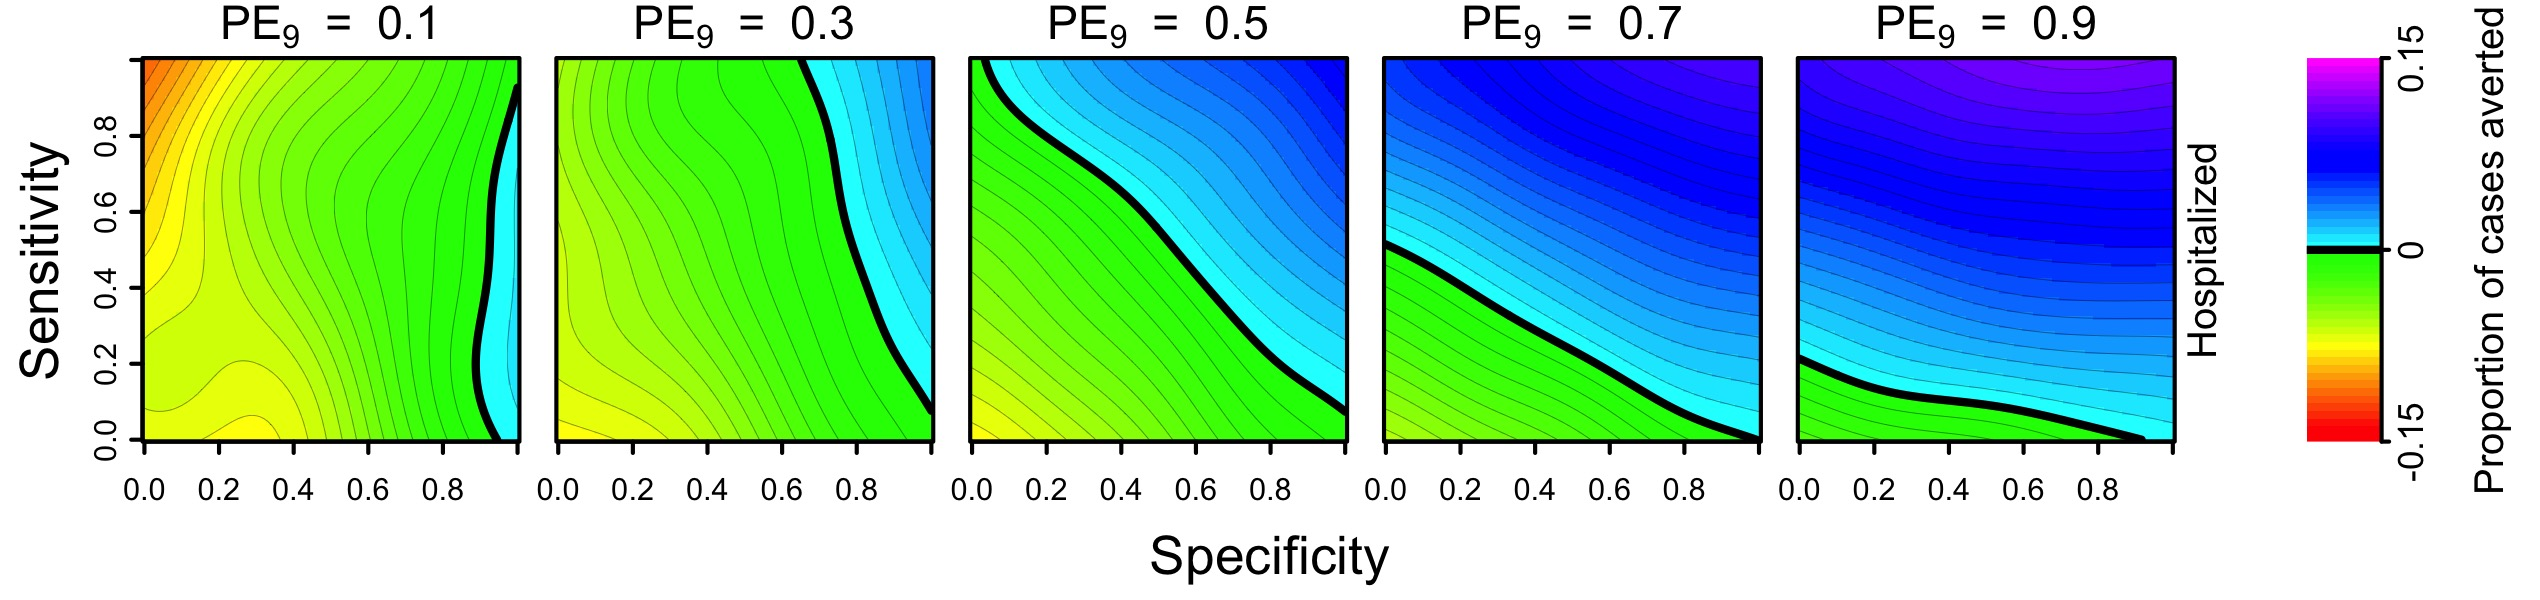
\includegraphics[width=.9\linewidth]{../analysis/figures/report_figure_cases_averted_heatmap_10y.jpeg}
\caption{Proportion of cases averted with pre-vaccination screening strategy with CYD-TDV over 10 years}
\label{fig-epi-benefits}
\end{figure}


\subsection{Cost-effectiveness of pre-vaccination screening strategies}
Out cost-effectiveness analysis suggests that the intervention would be cost-effective in Puerto Rico at the assumed price of the vaccine (70 USD) (Fig. \ref{fig-ICER}). Below 200 USD per fully vaccinated person, pre-vaccination screening would be cost-effective from a public payer perspective (ICER < 3 GDP per Capita). Very cost-effective scenarios could be achieved with a vaccine price below 95 USD per vaccinated individual. Also, at 18 USD per vaccinated individual, the costs of the intervention are equal to the costs without intervention (ICER = 0). Nonetheless, these cost-effectiveness thresholds depend on our assumptions of specificity and sensitivity of screening. 


\begin{figure}[H]
\centering 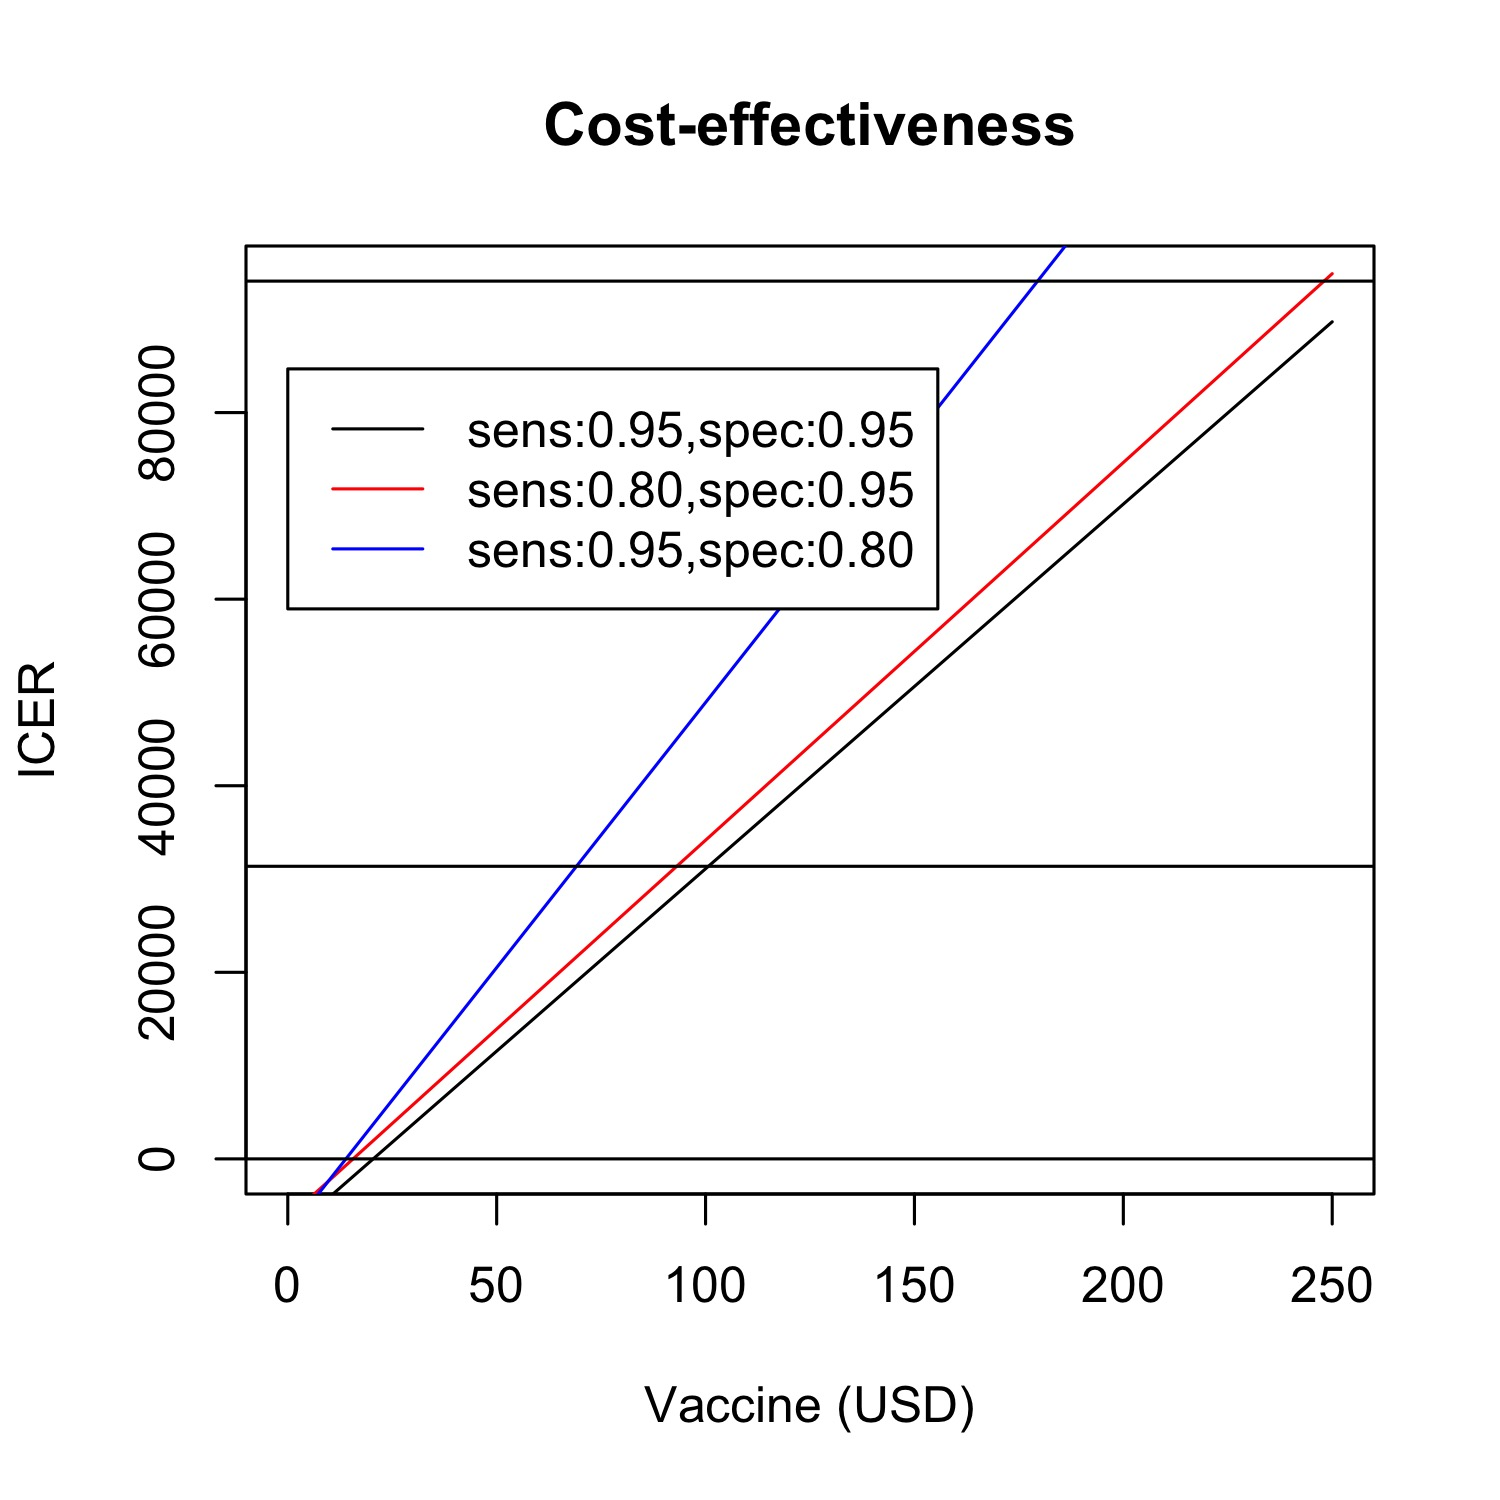
\includegraphics[width=.7\linewidth]{../analysis/figures/report_figure_ICER_PublicPayer_PuertoRico_10y.jpeg}
\caption{ICER of pre-vaccination screening strategy in Puerto Rico at different cost of vaccination (3 doses per person).}
\label{fig-ICER}
\end{figure}

\subsection{Tornado diagram and sensitivity analysis}
We varied the baseline value of five parameters of the cost-effectiveness analysis: sensitivity, specificity, PE9, vaccine cost for a fully vaccinated individual, and screening unit cost. The ranges of the parameter values are summarized in table \ref{table-tornado}.

%% Make sure this figure is updated every time the document is compiled (or at least for publication)
\begin{figure}[H]
\centering 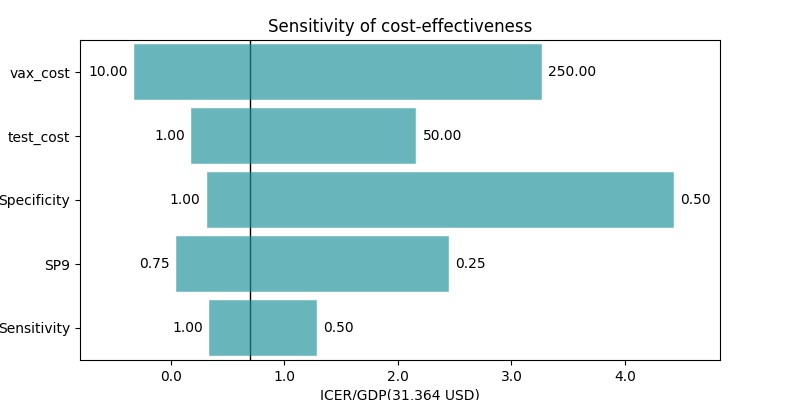
\includegraphics[width=.8\linewidth]{../analysis/figures/report_figure_tornado_diagram.jpeg}
\caption{ICER of pre-vaccination screening strategy in Puerto Rico at different cost of vaccination (3 doses per person).}
\label{fig-tornado}
\end{figure}

%% automatically insert results from R in here
\begin{table}[ht]
\centering
\begin{tabular}{|c|c|c|c|c|c|c|}
  \hline
parameter & min & max & ICER\_min & ICER\_max & ICER\_default & GDP \\ 
  \hline
Sensitivity & 0.50 & 1.00 & 32622.40 & 18452.13 & 22012.70 & 31364.60 \\ 
  SP9 & 0.25 & 0.75 & 69042.20 & 9161.02 & 22012.70 & 31364.60 \\ 
  Specificity & 0.50 & 1.00 & 131214.40 & 17682.60 & 22012.70 & 31364.60 \\ 
  test\_cost & 1.00 & 50.00 & 13438.97 & 60118.17 & 22012.70 & 31364.60 \\ 
  vax\_cost & 10.00 & 250.00 & -2279.54 & 94889.41 & 22012.70 & 31364.60 \\ 
   \hline
\end{tabular}
\caption{Sensitivity analysis of cost-effectiveness} 
\label{table-tornado}
\end{table}


\section{Discussion}
Assuming a moderate transmission intensity in Puerto Rico, we found that this intervention could be beneficial from the public health and individual perspective, conditioned to moderate values of sensitivity and high values of specificity. Compared to our previous simulation analysis for the Philippines and Brazil \cite{Espana2019Biorxiv}, the main differences of this analysis are the costs of treatment of dengue fever and severe dengue cases, which are based on studies from 2010. More recent estimates of this type of costs would refine the estimates of cost-effectiveness of p re-vaccination screening with CYD-TDV in Puerto Rico. 

 \bibliographystyle{vancouver}
 %% automatically copy updated .bib file from Dropbox/Literature directory
 \bibliography{Guido_Postdoc_Literature}
\end{document}
%%% Local Variables:
%%% mode: latex
%%% TeX-master: t
%%% End:
